\chapter{Angepasster Entwicklungsablauf}
\label{cha:angepasster_entwicklungsablauf}

\section{Grundlegende Gedanken zur Spielmechanik}
%\label{sec:}
Einer der wichtigsten Gedanken ist natürlich, wie bringe ich andere Menschen dazu Zeit und Geld in ein Spiel zu investieren. 

Kindliches Spielen, Fangen, bauen, kämpfen

Gewinnen macht spaß, besser noch es ist schwieriger gewesen (dominieren)

Spielkonzepte, Schach 

...
Spielkonzepte mixen
Doch ist nicht jede Idee praktikabel und umsetzbar oder wird vielleicht durch andere Ideen obsolet. [Zitat] Bsp.: Gibt man einem Spieler die Möglichkeit sich in Bestimmten Mustern über den Bildschirm zu bewegen und dem anderen Spieler die Fähigkeit großflächig schaden anzurichten, (Fußsoldat und Kampfjet) hat dieser einen unfairen Vorteil, der vielleicht auf den ersten Blick gar nicht auffällt. Daher muss man sich bei der Kombination verschiedener Spielelemente stets darüber im klaren sein, was man damit erreichen möchte...

\section{(Ursprüngliche) Konzeption}
%\label{sec:}
An dieser Stelle muss vorab gesagt werden, dass das Spiel anfangs als virtuelles Haustier geplant worden ist, die grundlegende Spielidee sich aber mit dem wachsenden Wissensstand mehr und mehr transformiert hat.
 
Diese Skizze ist eine der ersten von uns erstellten Skizzen zur Spielmechanik. Sie soll zeigen welche Features ursprünglich geplant wurden. Im Folgenden werden einzelne Punkte der Zeichnung erläutert um deren Sinn und Zweck zu klären.

Einer der wichtigsten Standpfeiler der Spielmechanik ist es, dass das Spiel nicht zeitintensiv ist. Es soll vollkommen ausreichen täglich nur einige Minuten im Spiel zu verbringen. Dies soll dabei helfen das Spielerlebnis über einen längeren Zeitraum zu vergrößern, da so die vorgegebene Story nicht einfach eben schnell innerhalb von einigen Stunden durchgespielt werden kann. Dieser Punkt hat auch die Entscheidung beeinflusst die gesamte Geschichte des Spiels Episodenbasiert zu machen.  Dadurch das die Hintergrundgeschichte und das aktuelle Geschehen in Einzelteilen nachgereicht werden kann verkürzt die Zeit der Entwicklung ungemein, da alle auftauchenden Personen
an verschiedenen Orten unterschiedliche Tiere in Verschiedenen Städten
-Diverse Boni bei Unterschiedlichen Geschäften
-Unterschiedliche Farben Items je nach Uhrzeit, Wetter, Umgebung
-Versteckte Items, Items pflanzen
-Reviere, Geofence markiert Zuhause, Tiere reagieren verschieden auf andere Tiere (Knurren, Schnuppern usw.)
-Laufweg analyse, Tiere freuen sich über neue Orte und verschiedene Geschwindigkeiten und können Spuren von anderen Tieren wahrnehmen
-Personen können Orte hinzufügen (User generated content)
-In Home Zones können die Pets ihre mobilen Endgeräte verlassen und den Rechner und andere mobile Geräte "besuchen".

\section{Elevator pitch zur Finanzierung}
%\label{sec:}
\url{http://www.slidefinder.net/n/nabc_need_approach_benefit_competition/33029996}

\subsection{Need:}
%\label{sec:}
Das Bedürfnis gebraucht zu werden - Diese Ursache liegt oft unbewusst in uns und ist deshalb gar nicht so leicht zu durchschauen. Fuer andere da sein zu können, gebraucht zu werden, helfen zu können – all das tut vielen Menschen sehr gut.
\url{http://www.zeitzuleben.de/2522-5-tipps-zum-nein-sagen/}
(echte Haustiere, Babyborn...)
Bedürfnis nach Abwechslung und Entertainment
Bedürfnis nach Belohnung
Bedürfnis nach Bewegung und Entdeckungen 
sociallife
Spiele sind da um der Realität zu entfliehen, etwas neues zu erleben,
den Entdeckertrieb zu fördern und belohnen den Spieler auch noch dabei.
Dabei wird man in den meisten Fällen aber leider von dem Computer oder der Spielekonsole an die eigenen vier Wände gebunden.
Somit leidet auch sehr oft das soziale Leben. 
Verantwortung lehren 
Leider sind viele Spiele nüchtern betrachtet eine reine Zeitverschwendung 
studien zu Intelligenz verbesserung oder agressions steigerung tauchen andauernd auf und werden wieder verworfen. 
Reine lernspiele oft langweilig. 
Was kann ein Spiel wirklich übermitteln?
Verantwortung 
-coolness Faktor 
-haustiere, items vergleichen 

\subsection{Approach:}
%\label{sec:}
virtuelles Haustier das den Besitzer braucht und durch örtlichen Bezug Abenteuer erleben kann 
Interaktion mit anderen Spielern sorgt für neue Wesen / neue Gegenstaende / Belohnungen 
Erfolge / Medaillen u. Ae. bei guter Pflege, entdeckte Orte oder anderer Tätigkeiten

\subsection{Benefits:} 
%\label{sec:}
spielerisches lernen von Verantwortung ohne groessere Schaeden
Community-Bildung durch die Spieler
Ermutigung die Wohnung zu verlassen
herausstechen aus der Masse durch besondere Monster / Gegenstaende
Competition:moderne loesungen 
Mobbles.... gibt sehr viele
Tamagotchi, Pokemon,
(Vielleicht mal \url{http://www.kickstarter.com/projects/1171494076/scriggles-ios-virtual-pet-game} anschauen 
sieht gar nicht schlecht aus, ist aber episch den bach runter gegangen)

\section{Evolution der Spieleidee} 
%\label{sec:}
Durch das Testen mehrerer Spiele, die sich mit dem Thema virtual pet beschäftigen sind wir zu dem Entschluss gekommen,  dass sich der größte teil der virtual pet spiele bzw. Lebenssimulationen einen ganz anderen Umfang als das von uns angestrebte ziel anpeilen. Wir sind ursprünglich davon ausgegangen, das die Lebenssimulationen wie bei den aus den 1990ern bekannten Tamagotchies einfach nicht optimal in die Neuzeit übertragen wurden, jedoch hat sich bei der tieferen Recherche ergeben, dass dieses genre jedoch nicht den umfang bietet ein Spiel zu entwickeln, das es schafft Spieler über einen längeren Zeitraum zu binden. Da die meisten Spieler schon nach wenigen Lebenszyklen das meiste solcher Spiele gesehen haben. Neue Items oder kleine mini Spielchen wie ein tic tac toe helfen dort auch nicht weiter. Da die Spiele damit im Grunde lediglich zu einer Minispiel-Sammlung aufgebläht werden und das eigentliche Spielprinzip dadurch mehr und mehr in den Schatten gestellt wird. Daher lag es auf der Hand das Thema von einer ganz anderen Seite her anzugehen. Wenn man das Spielkonzept durch Elemente aus rogue like game bekannten Titeln hinzufügt, erhält man plötzlich ein völlig neues und anderes Spielerlebnis.
Wie bereits im vorherigen Kapitel beschrieben, sollen Spiele, die sich nicht ihre eigene Kunst als Hauptziel setzen den Spieler fordern indem er in komplexen Situationen die bestmögliche Entscheidung treffen muss. Dies würde dazu führen, dass man nicht einfach nur sein Tier mit Nahrung versorgt, sondern darauf achten muss, was genau verfüttert wird. 
Auf der anderen Seite kann dies wiederum auch schnell frustrieren, da man auch aus Versehen das falsche Item benutzen kann und sich somit den weiteren Spielverlauf verbaut.
Ein Blick auf die finale Spiele Idee zeigt, wie sich diese Probleme umgehen lassen. 
Ein anderer punkt ist die schnelllebige zeit in der wir leben.

[1]
[1]

[1]
[1]
[1]


\section{Definition der Spielmechanik} 
%\label{sec:}
\textbf{7 Tage Lebenszeit!}
Victory Points: 
\begin{equation}
5*5=16
\end{equation}

%\begin{tikzpicture}
%\begin{axis}
%    \addplot (\x,1440+\x *800);
%\end{axis}
%\end{tikzpicture}

%\begin{tikzpicture}
%  \draw[->] (-3,0) -- (4.2,0) node[right] {$x$};
%  \draw[->] (0,-3) -- (0,4.2) node[above] {$y$};
%  \draw[scale=0.5,domain=-3:3,smooth,variable=\x,blue] plot ({\x},{sqrt(\x)});
%  \draw[scale=0.5,domain=-3:3,smooth,variable=\y,red]  plot ({\y*\y},{\y});
%\end{tikzpicture}


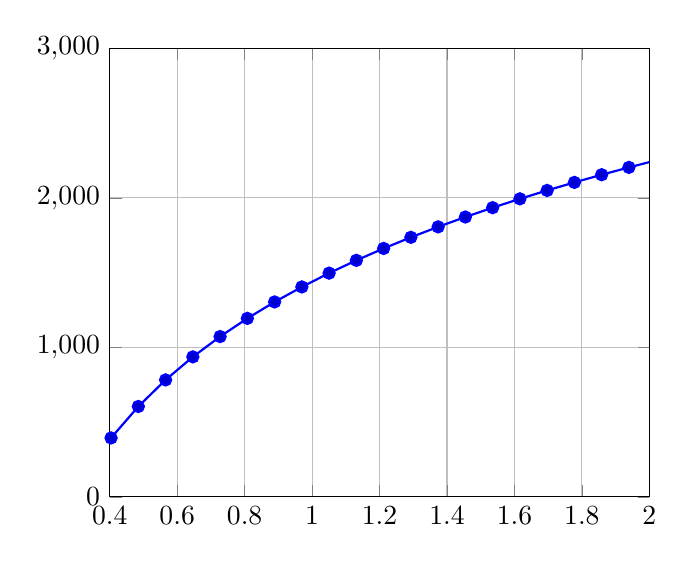
\begin{tikzpicture}
\begin{axis}[domain=0:8,
 samples=100,
 xmin=.4,   xmax=2,
	ymin=0,   ymax=3000,
 % enlarge x limits=false,
  grid=both,
  %no markers,
  %axis equal
  ]
  
  %\draw[->] (-3,0) -- (4.2,0) node[right] {$x$};
  %\draw[->] (0,-3) -- (0,4.2) node[above] {$y$};
\addplot +[thick] {1440+log2(x)*800};
\end{axis}
\end{tikzpicture}



1. Sieg: 1440+log(2, 1.0)*800 = 1440
2. Sieg: 1440+log(2, 0.8)*800 = 1182
3. Sieg: 1440+log(2, 0.6)*800 = 850
4. Sieg: 1440+log(2, 0.4)*800 = 382 Nach dem vierten Sieg werden immer 382 Punkte gutgeschrieben

Highscore: Lebenszeit in Minuten + Victory Points

MaxLebenszeit: (7*24*60 = 10080) 
Items: +50,  +25, +13, +7
Stärke – Strenght 			hantel
Intelligenz – Intelligence 		buch
Geschicklichkeit – Dexterity	werkzeug
Charisma – Charisma		spiegel
Glück – Luck				kleeblatt 
(generierung)Werte werden zufällig aus dem PetDBSchema ermittelt 

kampf 
spieler wählt attribut
wenn attribut = max von pet dann multiplikator
spieler + max von pet, wird verglichen
werte schätzen 

Es wird geschlagen oder gestochen
Ältere tiere gewinnen
- NPC? > Arenen
- 5 Abilities (St‰, Ges, Int, Cha, Glk)
- 1. Tier am Anfang; randomized Ab.

- Delta/Ability: 100 [1-100]
- Farbe wird durch Werte bestimmt
---
- Arena mit passiven F‰h. --> Arena

- Lebenszeit = 7 Tage = 168 Stds oder 10080 Min
- Siegpunkte = -log2(anz. Siege) [1Sieg ~ 1440 Min t‰glicher reset des log]
- Sieg in Arena (Arenabesitzer) = 1/4 der Siegpunkte
- Highscore = Lebenszeit + Siegpunkte
- Siege: 7-21 durchschn. pro Woche

- Ein Kampf pro Tag pro Arena (kein Farmen)
- Niederlage: kein Malus (kostet Zeit)
- Items: +50 +25 +13 +
	Hantel > Stä
	Buch > Int
	Werkzeug > Ges
	Spiegel > Char
	Kleeblatt > Gl
+50 wenn vorteil
Tier 1 

	S 	I 	G 	C 	Gl

	44	65	74	89	12

Tier 2
	S 	I 	G 	C 	Gl
	55	94	70	61	49


Werte werden nach und nach aufgedeckt (zufällig)



[1]	M. Fogus, Functional JavaScript. “O'Reilly Media, Inc.,” 2013.
